\section{Feature extraction}
\label{feature-extraction}

This Sections presents the original dataset structure and the 
steps followed to create training and test sets from it.

Note that the models mentioned in this section, for the first and 
extended datasets are
three layers \emph{multilayer perceptrons}, 
a feed forward neural network where each layer 
is densely connected  to the following, 
with a reasonable number of neurons, trained 
for 100 epochs with default parameters for the \emph{stochastic gradient 
descent optimizer}.~\cite{mlp}\cite{sgd}\\
A \emph{convolutional neural network}, a network with 
a series of convolutional and pooling layers, followed by 
some densely connected ones, is applied to the image dataset, trained for 10 epochs
with default parameters for the Adam optimizer.~\cite{cnn} \\
For all datasets, the accuracy mentioned is computed with a \emph{cross-validation} 
approach.~\cite{cross}\\

A deeper discussion about the models structure as well as the validation
techniques used in the project can be found at Section \vref{model-definition}.

\subsection{Dataset structure}
\label{dataset-structure}

The UrbanSound8k dataset contains ten folds of audio samples, each one about 
four seconds long. The samples are divided in ten classes.\\
From the total of ten folds, the number one, two, three, four and six 
are taken as a training set, the others are each one a test set.
For this reason the following count about class numerosity considers
only the five training folds.

\begin{center}
    \begin{tabular}{ |l|c| } 
        \hline
        Class name & Number of samples \\
        \hline
        air conditioner & 500 \\
        car horn & 208 \\
        children playing & 500 \\
        dog bark & 500 \\
        drilling & 500 \\
        engine idling & 517 \\
        gun shot & 190 \\
        jackhammer & 548 \\
        siren & 536 \\
        street music & 500 \\
        \hline
    \end{tabular}
\end{center}

The table shows a clear class imbalance. In particular, the classes 
\emph{car horn} and \emph{gun shot} are not as numerous as the others. 
This can lead to poor performances on the these two categories, it is
therefore taken 
into consideration with training. 

The following table shows the number of samples in the training set and 
the various test sets.

\begin{center}
    \begin{tabular}{ |l|c| } 
        \hline
        Dataset & Number of samples \\
        \hline
        Training set & 4499 \\
        Test set 5 & 936 \\
        Test set 7 & 838 \\
        Test set 8 & 806 \\
        Test set 9 & 816 \\
        Test set 10 & 837 \\
        \hline
    \end{tabular}
\end{center}
All the operations on the datasets are performed with \emph{Pandas} library.~\cite{pandas}

\subsection{First dataset}
\label{first}
Extracting features from audio files is not straightforward, nonetheless there 
are a collection of audio characteristics that are commonly used in audio machine learning 
applications.~\cite{features}

To extract information from audio files \emph{Librosa} is used.~\cite{librosa}
The library provides many methods to choose from,
to keep it simple, for the first try with this dataset, the extracted features 
are these three ones: 
\begin{enumerate}
    \item \emph{Mel-frequency cepstral coefficients}: the first 20 coefficients 
    are extracted;
    \item \emph{Chromagram}: the first 12 chromas are considered;
    \item \emph{Root-mean-square}.
\end{enumerate}
Method parameters that are not specified in the above list, are left on their default values.
Each feature consists of an array of arrays containing measurements. 
A series of functions are applied to each sub-array and results 
are concatenated in a final feature vector. 
The functions applied are \emph{minimum}, \emph{maximum}, \emph{mean} 
and \emph{median} from the \emph{Numpy} library.~\cite{numpy}

This approach results in 132 components feature vectors.

\paragraph{Parallelizing feature extraction}
Extracting the three features listed above is really intensive 
but the task is easily parallelizable, in fact, each file is independent 
from one another.

For this purpose \emph{Dask} is used to speed up the computation and 
extract features from audio files in a multi-processing fashion.~\cite{dask}
The main idea is to build an execution plan, where each audio file 
is managed in parallel by a collection of workers. 
Improvement is great as the time to process a single fold 
is cutted into a third.

\paragraph{Feature scaling}
After testing some neural networks on the first dataset results 
are not promising. One of the reasons is the big difference in 
ranges among feature vector components, for instance, 
some audio characteristics are in the order of thousands while others 
range between zero and one.

To mitigate this effect a \emph{StandardScaler} with default parameters from \emph{scikit learn} is applied.~\cite{scaler}
The result is a dataset where each feature has more or less a distribution 
centered in zero with unit variance.
This leads to an improvement on the results using the same
model as before. 


\subsection{Extended dataset}
\label{extended-dataset}

Results using the three features named in the previous Subsection 
are promising but not enough, thus, to improve accuracy on the training set, 
new audio characteristics are extracted, namely:
\begin{enumerate}
    \item \emph{Zero-crossing rate};
    \item \emph{Roll-off frequency};
    \item \emph{Spectral flux onset strength}.
\end{enumerate}
As before methods parameters are left on default, but 
this time \emph{standard deviation} is added to
the previous functions \emph{minimum}, \emph{maximum}, \emph{mean} 
and \emph{median}. Each one is applied to the feature sub-vectors and 
results are concatenated, leading to a total of 180 features for each audio file.
Scaling yields to promising results on the first dataset, 
so the same approach is applied to the extended one.

After testing a network on the new training set 
we can see a better accuracy.

\paragraph{Feature selection}
Adding new features can lead to better results 
in the end but they all need to be useful to the model.
For this reason the extended dataset is subject of some experiments 
with feature selection, in particular \emph{PCA} algorithm from scikit
learn is applied.~\cite{pca}

The main idea is to select a reduced number of features from the total, 
loosing as little information as possible. This approach often leads to better results, 
as useless features are discarded.

The method used to select features offers the possibility to specify how much 
variance to preserve in the reduced dataset, this means that the number of 
components is not given explicitly, indeed we try to preserve 99 percent of the original variance.

This technique resulted in 102 features, unfortunately, a model applied to this new dataset 
failed to reach the performances obtained by the previous one, nonetheless, performances
improved with respect to the scaled dataset.

\subsection{Image dataset}
A completely different approach is followed this time to represent audio files 
as images, to later apply a convolutional neural network.

\paragraph{Audio as an image}
Representing an audio as an image is not straightforward but can be done after 
some preprocessing.
The main idea is to use audio features and consider them in a two dimensional 
space, where the value of a single cell can be viewed as a pixel.
Note that some features are well suited for this kind of representation, for instance, 
some of the previously extracted ones are given in output as a two dimensional vector.

Usually, an image has three channels, red, green and blue, but 
image classification on grayscale images, with one single channel 
is also relevant. This means that one can extract multiple features and view them 
as different channels, or choose only one to have the equivalent of a grayscale image.

\paragraph{Short time Furier Transform}
For this try with image classification the Short-time Furier transform 
is extracted from the audio files, and then used as a single channel image. 
In particular, we extract 128 intervals with the \emph{stft} function from Librosa, and, to accomodate 
the different lenghts of audio in the dataset, pad the result to 256 wide vectors.
The result is an $128 \times 256$ image for each sample. Figure \ref{img}
shows an example of an image obtained for each class.

\begin{figure}
    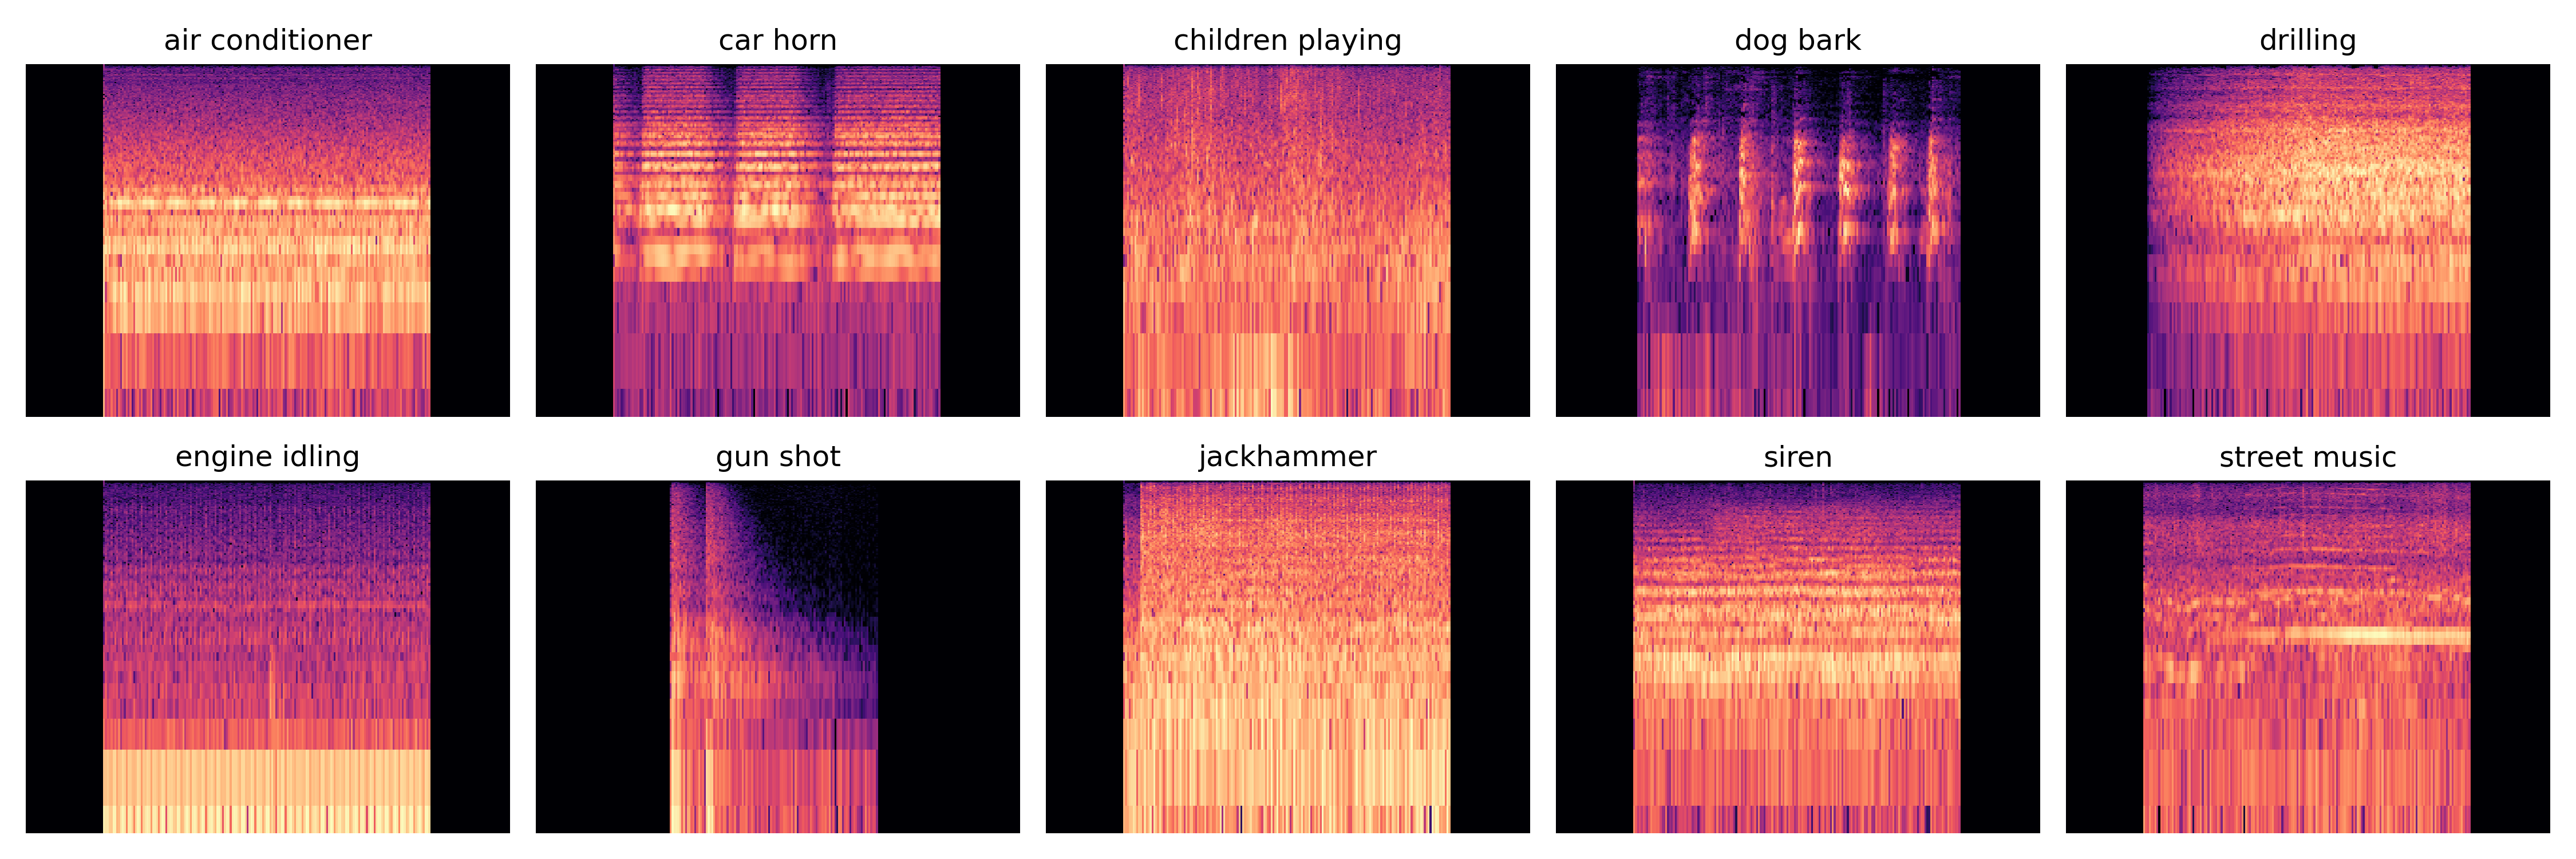
\includegraphics[width=\textwidth]{images/class_images.png}  
    \caption{Short time Furier transform on samples coming from each class.
    The scale on the Y axis is logarithmic, the X axis represent time and 
    the black portion on the edges is due to the applied padding.}  
    \label{img}
\end{figure}

We can see some difference between the classes, for instance, the \emph{dog barking}
shows short repeated sounds, \emph{gun shot} has a declining intensity, while \emph{air conditioner}
is constant. The hope is that those subtle differences are enough lo learn and classify.

\paragraph{Scaling pixel values}
Scaling techniques  are usually applied even to images to prevent high disparities 
among pixel value ranges, for this reason a Standard scaler with default parameters is 
once again applied to the training set to mitigate this effect.
We can not apply it directly to the images, as they are two dimensional, but we can 
flatten the pixel arrays, apply scaling and reshape them in the original $128 \times 256$ format.

Testing a convolutional network 
on the image dataset gives results that are comparable to the ones obtained on the initial scaled training 
set, discussed at Subsection \vref{first}.
\newpage